% chap02sec01
\section{Finite, countable, and uncountable sets}

We begin this section with a definition of the \myKeywordblue{function} concept.

\mybox{
    Function

    \url{https://mathworld.wolfram.com/Function.html}


A function is a relation that uniquely associates members of one set with members of another set. 
More formally, a function from $A$ to $B$ is an object $f$ such that every $a$ in $A$ is uniquely associated with an object $f(a)$ in $B$. 
A function is therefore a many-to-one (or sometimes one-to-one) relation. 
The set $A$ of values at which a function is defined is called its domain, 
while the set $f(A)$ subset $B$ of values that the function can produce is called its range. 
Here, the set $B$ is called the codomain of $f$.

In the context of univariate, real-valued functions $f:A \subset \R\rightarrow \R$, 
the fact that domain elements are mapped to unique range elements can be expressed graphically by way of the vertical line test.

In some literature, the term 
``map''
 is synonymous with function. 
Some caution must be exhibited, however, as it is not uncommon for the term map to denote a function with some sort of unspoken regularity assumption, 
e.g., in point-set topology, where 
``map''
 sometimes refers to a function which is continuous with respect to some topology.
}

%  too long notes out side box
\begin{center}
    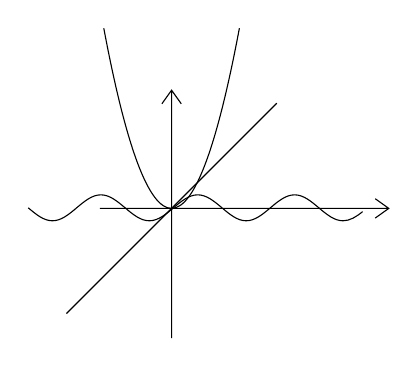
\begin{tikzpicture}[x=0.7pt,y=0.7pt,yscale=-1,xscale=1]
    %uncomment if require: \path (0,300); %set diagram left start at 0, and has height of 300
    
    %Shape: Axis 2D [id:dp21476035781689284] 
    \draw  (165.52,146.23) -- (314.72,146.23)(202.6,85.23) -- (202.6,213.23) (307.72,141.23) -- (314.72,146.23) -- (307.72,151.23) (197.6,92.23) -- (202.6,85.23) -- (207.6,92.23)  ;
    %Shape: Wave [id:dp7563242846602689] 
    \draw   (128.6,145.93) .. controls (132.68,149.37) and (136.58,152.63) .. (141.1,152.63) .. controls (145.62,152.63) and (149.52,149.37) .. (153.6,145.93) .. controls (157.68,142.5) and (161.58,139.23) .. (166.1,139.23) .. controls (170.62,139.23) and (174.52,142.5) .. (178.6,145.93) .. controls (182.68,149.37) and (186.58,152.63) .. (191.1,152.63) .. controls (195.62,152.63) and (199.52,149.37) .. (203.6,145.93) .. controls (207.68,142.5) and (211.58,139.23) .. (216.1,139.23) .. controls (220.62,139.23) and (224.52,142.5) .. (228.6,145.93) .. controls (232.68,149.37) and (236.58,152.63) .. (241.1,152.63) .. controls (245.62,152.63) and (249.52,149.37) .. (253.6,145.93) .. controls (257.68,142.5) and (261.58,139.23) .. (266.1,139.23) .. controls (270.62,139.23) and (274.52,142.5) .. (278.6,145.93) .. controls (282.68,149.37) and (286.58,152.63) .. (291.1,152.63) .. controls (294.73,152.63) and (297.96,150.53) .. (301.2,147.92) ;
    %Shape: Parabola [id:dp3307772220116144] 
    \draw   (167.6,53.23) .. controls (190.93,177.23) and (214.27,177.23) .. (237.6,53.23) ;
    %Straight Lines [id:da017349586183422416] 
    \draw    (148.3,200.53) -- (256.9,91.93) ;
    
\end{tikzpicture}
\end{center}

Examples of functions over the reals $\R$ include $\sin x$ (many-to-one), $x$ (one-to-one), $x^2$ (two-to-one except for the single point $x=0$), etc.

Unfortunately, the term ``function'' is also used to refer to relations that map single points in the domain to possibly multiple points in the range. 
These ``functions'' are called multivalued functions (or multiple-valued functions), and arise prominently in the theory of complex functions, 
where the presence of multiple values engenders the use of so-called branch cuts.

Several notations are commonly used to represent (non-multivalued) functions. 
The most rigorous notation is $f:x\rightarrow f(x)$, which specifies that f is function acting upon a single number $x$ (i.e., f is a univariate, or one-variable, function) and returning a value $f(x)$. 
To be even more precise, a notation like ``$f:R\rightarrow R$, where $f(x)=x^2$''
 is sometimes used to explicitly specify the domain and codomain of the function. 
The slightly different 
``maps to''
 notation $f:x|\rightarrow f(x)$ is sometimes also used when the function is explicitly considered as a 
``map''.




\mybox{
    Generally speaking, the symbol $f$ refers to the function itself, while $f(x)$ refers to the value taken by the function when evaluated at a point $x$. 
However, especially in more introductory texts, the notation $f(x)$ is commonly used to refer to the function $f$ itself (as opposed to the value of the function evaluated at $x$). 
In this context, the argument $x$ is considered to be a dummy variable whose presence indicates that the function $f$ takes a single argument (as opposed to $f(x,y)$, etc.). 
While this notation is deprecated by professional mathematicians, it is the more familiar one for most nonprofessionals. 
Therefore, unless indicated otherwise by context, the notation $f(x)$ is taken in this work to be a shorthand for the more rigorous $f:x\rightarrow f(x)$.
}

\begin{mydef}
    \label{mydef:2.1}
    Consider two sets $A$ and $B$, whose elements may be any objects whatsoever, 
    and suppose that with each element $x$ of $A$ there is associated, 
    in some manner, an element of $B$, which we denote by $f(x)$. 
    Then $f$ is said to be a \myKeywordblue{function} from $A$ to $B$ (or a \myKeywordblue{mapping} of $A$ into $B$). 
    The set $A$ is called the \myKeywordblue{domain} of $f$ (we also say $f$ is defined on $A$), 
    and the elements $f(x)$ are called the \myKeywordblue{values} of $f$.
    The set of all values of $f$ is called the \myKeywordblue{range} of $f$.
\end{mydef}
\mybox{\myKeywordblue{Codomain}:  A set within which the values of a function lie (as opposed to the range, which is the set of values that the function actually takes). 

\myKeywordblue{Range}:   If $f:D\rightarrow Y$ is a map (a.k.a. function, transformation, etc.) over a domain $D$, 
then the range of $f$, also called the image of $D$ under $f$, 
is defined as the set of all values that $f$ can take as its argument varies over $D$, i.e.,
\begin{equation*}
    \operatorname{Range}(f)=f(D)={f(\mathbf{X}):\mathbf{X} \in D}.
\end{equation*}

Note that among mathematicians, the word 
``image''
 is used more commonly than 
``range.''


The range is a subset of $Y$ and does not have to be all of $Y$.

Unfortunately, term 
``range''
 is often used to mean domain--its precise opposite--in probability theory, with Feller (1968, p.200) and Evans et al. (2000, p.5) calling the set of values that a variate $X$ can assume (i.e., the set of values $x$ that a probability density function $P(x)$ is defined over) the 
``range''
, denoted by $R_X$ (Evans et al. 2000, p.5).

Even worse, statistics most commonly uses 
``range''
 to refer to the completely different statistical quantity as the difference between the largest and smallest order statistics. In this work, this form of range is referred to as 
``statistical range.''
 
}

\begin{mydef}
    \label{mydef:2.2}
    Let $A$ and $B$ be two sets and let $f$ be a mapping of $A$ into $B$.
    If $E \subset A$, $f(E)$ is defined to be the set of all elements $f(x)$, for $x \in E$. We call $f(E)$ the image of $E$ under $f$. In this notation, $f(A)$ is the range of $f$. It is clear that $f(A) \subset B$. If $f(A) = B$, we say that $f$ maps $A$ \myKeywordblue{onto} $B$. (Note that, according
    to this usage, \myKeywordblue{onto} is more specific than \myKeywordblue{into}.)
    % \mybox{onto 满射? into 映射?} 
    
    \url{https://www.mathsisfun.com/sets/injective-surjective-bijective.html}
    \begin{figure}[htbp]
        \centering
        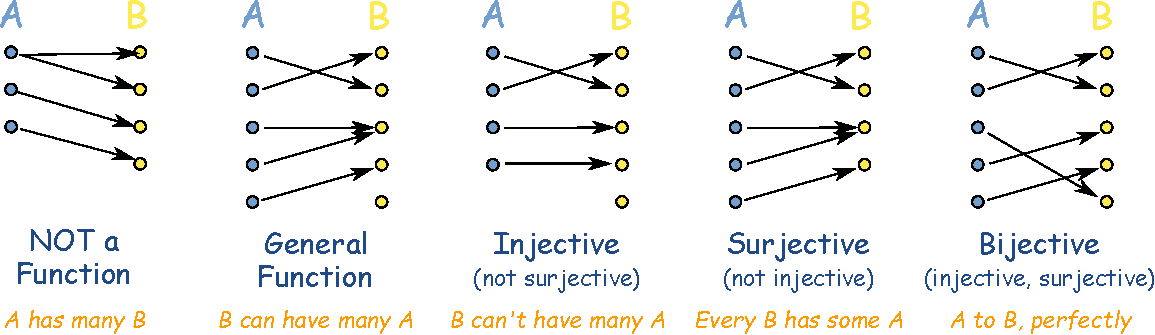
\includegraphics[width=0.7\linewidth]{pic/function-mapping.pdf}
        \caption{function-mapping}
        \label{fig:function-mapping}
    \end{figure}
        \mybox{
        injective ``one-to-one'' \\    
        surjective ``onto'' \\
        bijective both injective and surjective. \\
        my question: what is ``into''?
        } 

    If $E \subset B$, $f^{-1}(E)$ denotes the set of all $x \in A$ such that $f(x)\in E$. We call $f^{-1}(E)$ the \myKeywordblue{inverse image} of $E$ under $f$. If $y \in B$, $f^{-1}(y)$ is the set of all $x \in A$ such that $f(x) =y$. If, for each $y\in B$, $f^{-1}(y)$ consists of at most one element of $A$, then $f$ is said to be a 1-1 (\myKeywordblue{one-to-one}) mapping of $A$ into $B$. This may also be expressed as follows: $f$ is a 1-1 mapping of $A$ into $B$ provided that $f(x_1) \neq f(x_2)$ whenever $x_1 \neq x_2$, $x_1 \in A$, $x_2 \in A$.

    (The notation $x_1 \neq x_2$, means that $x_1$ and $x_2$ are distinct elements; otherwise we write $x_1 = x_2$.)
\end{mydef}

\begin{mydef}
    \label{mydef:2.3}
    If there exists a 1-1 mapping of $A$ \myKeywordblue{onto} $B$, we say that $A$ and $B$ can be putin 1-1 correspondence, or that $A$ and $B$ have the same cardinal number, or, briefly, that $A$ and $B$ are equivalent, and we write $A\sim B$. This relation
    clearly has the following properties :

    It is reflexive: $A\sim A$.

    It is symmetric: If $A\sim B$, then $B\sim A$.

    It is transitive: If $A\sim B$ and $B\sim C$, then $A\sim C$.

    Any relation with these three properties is called an equivalence relation.    
\end{mydef}
\mybox{等价关系:
reflexive   自反性,
symmetric   对称性,
transitive  传递性.

集合等势是一种等价关系, 其满足自反性, 对称性, 传递性.}

\begin{mydef}
    \label{mydef:2.4}
    $\forall n\in \mathbb{N}^+$, $J_n = \{1,2,...,n\}$, $J = \{1,2,...,n,...\}$, (set consisting of all positive integers).

    $A$ is finite, $A\sim J_n$ for some n,

    $A = \varnothing$. empty set is also considered to be finite.

    $A$ is infinite, $A$ is not finite.

    $A$ is countable, $A \sim J$
    
    $A$ is uncountable. $A$ is neither finite nor countable.

    countable set and finite set are called at most countable.
\end{mydef}

\mybox{
    \begin{equation*}
        \left\{
        \begin{array}{lll}
        finite & A\sim J_n\\
        infinite &\left\{
            \begin{array}{ll}
                countable& A\sim J\\
                uncountable& \\
            \end{array}
        \right.
        \end{array}
        \right.
    \end{equation*}
    % todo 添加tikz注释
}

countable sets, enumerable, denumerable.

$A, B \in$ finite set\\
$A\sim B$ $\Longleftrightarrow$ $A, B$ contains same number of elements

$A, B \in$ infinite set\\
same number or elements? vague\\
1-1 correspondence. retains its clarity.

\begin{newexample}
    $f:J\rightarrow A$
    \begin{equation*}
        f(n) = \left\{
            \begin{array}{ll}
                \cfrac{n}{2} & (n \text{  even})\\
                -\cfrac{n-1}{2} & (n \text{  odd})
            \end{array}
        \right.
    \end{equation*}
\end{newexample}
\mybox{$f(n)=(-1)^n\left\lfloor \cfrac{n}{2} \right\rfloor $}

\begin{myremark}
    a finite set cannot be equivalent to one of its proper subsets, but it's possible for infinite sets.
\end{myremark}

$J = 1,2,3,4,...$, $A = 0,1,-1,2,-2,...$,$J, A$are infinite sets, $J \subset A$.\\
but there exist a function $f:J\rightarrow A$, $J \sim A$

\begin{mydef}
    \label{mydef:2.7}
    $f(x)$, $x\in J = \mathbb{N}^+$.\\
    $\{x_n\}$, $x_1,x_2,x_3,...$\\
    $x_n$, terms of the sequence.\\
    $\forall n\in J$, $x_n\in A$, $\{x_n\}$ is a sequence in $A$, or a sequence of elements of $A$.
\end{mydef}

every countable set is range of a sequence of distinct terms.
the elements of any countable set can be ``arranged in a sequence''.
replace $J(\mathbb{N}^+)$ by $\mathbb{N} = \{x|, x\in Z,x \geq 0\}$, start with $0$ rather than $1$.

\begin{thm}
    \label{thm:2.8}
    Every infinite subset of a countable set $A$ is countable
\end{thm}

$E\subset A$. $E$ is infinite. 
To prove $E$ is countable, we need a 1-1 correspondation of $J$ to $E$, $f:J\rightarrow E$.
\mybox{
    my first guess is $A$ is a countable set, $A\sim J$ (by def).
    $\exists$ 1-1 mapping $g:$ $J$ onto $A$.
    $x\in J$, $g(x)\in A$.
    $E\subset A$, $\exists  g(x)\in E$.
    $g(x_i)\in E$, $x_i\in J$, $g:J\rightarrow E$.\\
    再证 $x_i$ 不是有限的. $E$ is infinite, there exist infinite $g(x_i)\in E$. $\because g$ is a 1-1 mapping, $\{x_i\}$ is infinite. $\therefore J\sim E$.
}

\begin{proof}
    Suppose $E\subset A$, $E$ is infinite. 
    arrange the elements $x$ of $A$ in a sequence $\{x_n\}$ of a distinct elements. Construct a sequence $n_k$ as follows.\\
    Let $n_1$ be the smallest positive int, s.t. $x_{n_1}\in E$.
    Having chosen $n_1,...n_{k-1}$,$(k=2,3,...)$, let $n_k$ be the smallest integer greater than $n_{k-1}$, s.t. $x_{n_k} \in E$.\\
    Putting $f(k) = x_{n_k}$, $f:J\rightarrow E$ is a 1-1 mapping.
\end{proof}

Countable sets represent the ``smallest'' infinity.

No uncountable set ca be a subset of a countable set.

\mybox{
    rudin 这里尝试区分实无穷与浅无穷, 
    使用集合的势来说明更为具体, 全体整数组成的集合为 ``最小'' 的无穷大, 
    其势为$\aleph_0$, 康托尔使用一一对应关系作为无穷集合之间的等价关系.
    }

\begin{mydef}
    \label{mydef:2.9}
    $\forall \alpha\in A$, $E_\alpha \subset \Omega$, $\{E_\alpha\}$ debites elements of $E_\alpha$. 
    collection of sets (or family of sets)  
    \mybox{sets of sets sounds strange}  
    union
    \begin{equation}
        \label{eq:2.1}
        S = \bigcup_{\alpha\in A} E_\alpha
    \end{equation}
    if $A$ consists of the integers $1,2,...,n$.
    \begin{equation}
        \label{eq:2.2}
        S = \bigcup_{m=1}^n E_m
    \end{equation}
    \begin{equation}
        \label{eq:2.3}
        S = E_1 \bigcup E_2 \bigcup \cdots \bigcup E_n.
    \end{equation}
    if $A$ is the set of all positive integers.
    \begin{equation}
        \label{eq:2.4}
        S = \bigcup_{m=1}^{\infty} E_m.
    \end{equation}
    intersection
    \begin{equation}
        \label{eq:2.5}
        P = \bigcap_{\alpha\in A} E_\alpha
    \end{equation}
    \begin{equation}
        \label{eq:2.6}
        S = \bigcap_{m=1}^n E_m = E_1 \cap E_2 \cap \cdots \cap E_n.
    \end{equation}
    \begin{equation}
        \label{eq:2.7}
        S = \bigcap_{m=1}^{\infty} E_m.
    \end{equation}

    $A$ and $B$ intersect if $A\bigcap B$ is not empty, otherwise they are disjoint.
\end{mydef}

\begin{newexample}
    % some example of set relation
    \begin{asparaenum}[(a)]
        \item Suppose $E_1$ consists of $1,2,3$ and 
        $E_2$ consists of $2,3,4$.
        Then $E_1 \cup E_2$ consists of $1,2,3,4$,
        whereas $E_1 \cap E_2$ consists of $2,3$.
        \item Let $A$ be the set of real number $x$ such that $0< x\leq 1$. 
        For every $x \in A$, let $E_x$ be the set of real numbers $y$ such that $0 < y < x$. Then 
        \begin{asparaenum}[(i)]
            \item \[E_y \subset E_x \text{ if and only if } 0 < x \leq z \leq 1;\] 
            \item \[\bigcup_{x\in A}E_x = E_1;\]
            \item \[\bigcap_{x\in A}E_x \text{ is empty};\]
        \end{asparaenum}
        (i) and (ii) are clear.
        To prove (iii), we note that for every $y>0$, $y \not\in E_x$ if $x < y$. 
        Hence $y \not\in \cap_{x\in A}E_x$.
    \end{asparaenum}
\end{newexample}

\begin{myremark}
    Many properties of unions and intersections are quite similar to those of sums and products; in fact, the words sum and product were sometimes used in this connection, and the symbols $\sum$ and $\prod$ were written in place of $\bigcup$ and $\bigcap$.
\end{myremark}

The commutative and associative laws are trivial:
\begin{align}
        A \cup B &= B \cup A; &
        A \cap B &= B \cap A \label{eq:2.8} \\
        \left(A \cup B\right) \cup C &= A \cup \left(B \cup C\right); &
        \left(A \cap B\right) \cap C &= A \cap \left(B \cap C\right);\label{eq:2.9}
\end{align}

Thus the omission of parentheses in \ref{eq:2.3} and \ref{eq:2.6} is justified.

The distributive law also holds:
\begin{equation}
    \label{eq:2.10}
    A \cap \left( B \cup C\right) = 
    \left(A \cap B\right) \cup \left(A \cap C\right).
\end{equation}
To prove this, let the left and right members of \ref{eq:2.10} be denoted by $E$ and $F$, respectively.

Suppose $x \in E$. Then $x \in A$ and $x \in B \cup C$, that is, $x \in B$ or$ x \in C$ (possibly both). Hence $x \in A\cap B$ or $x \in A\cap C$, so that $x \in F$. Thus $E \subset F$.

Next, suppose $x \in F$. Then $x \in A\cap B$ or $x \in A\cap C$. That is, $x \in A$, and $x \in B\cup C$. Hence $x \in A\cap \left(B \cup C\right)$, so that $F \subset E$.

It follows that $E = F$.

We list a few more relations which are easily verified:

\begin{align}
    A \subset A \cup B, \label{eq:2.11}\\
    A \cap B \subset B, \label{eq:2.12}
\end{align}

If $0$ denotes the empty set, then
\begin{equation}
    \begin{array}{cc}
        A \cup 0 = A, & A \cap 0 = 0.
    \end{array}
\end{equation}
If $A \subset B$, then
\begin{equation}
    \begin{array}{cc}
        A \cup B = B, & A \cap B = A.
    \end{array}
\end{equation}

\mybox{现在一般使用 $\varnothing$ 指代空集}


\begin{thm}
    \label{thm:2.12}
    Let $\{E_n\}, n=1,2,3,...,$ be a sequence of countable sets, and put
    \begin{equation}
        \label{eq:2.15}
        S = \bigcup_{n=1}^{\infty} E_n.
    \end{equation}
    Then S is countable.
\end{thm}
\mybox{
    将 $E_n$ 按顺序排成一张表格, 按反对角线重新排列成新的序列, 
    得到 $T$, $S\sim T$.
    $S$ is at most countable.
    同时存在无限集合(infinite set) $E_1$, $E_1 \subset S$, 
    $S$ is countable.
}

\begin{proof}
    Let every set $E_n$ be arranged in a sequence $\sequence{x_{nk}}$, 
    $k = 1,2,3,\dots$,
    and consider the infinite array
    \begin{equation}
        \label{eq:2.16}
        \begin{array}{ccccc}
            x_{11} & x_{12} & x_{13} & x_{14} & \cdots \\  
            x_{21} & x_{22} & x_{23} & x_{24} & \cdots \\  
            x_{31} & x_{32} & x_{33} & x_{34} & \cdots \\  
            x_{41} & x_{42} & x_{43} & x_{44} & \cdots \\  
            \cdots & \cdots & \cdots & \cdots & \cdots \\
        \end{array}
    \end{equation}
    in which the elements of $E_n$ form the $n$th row. 
    The array contains all elements of $S$.
    As indicated by the arrows, 
    these elements can be arranged in a sequence
    \begin{equation}
        \label{eq:2.17}
        x_{11};
        x_{21}, x_{12};
        x_{31}, x_{22}, x_{13};
        x_{41}, x_{32}, x_{23}, x_{14};
        \cdots
    \end{equation}
    
    If any two of the sets En have elements in common, 
    these will appear more than once in (\ref{eq:2.17}). 
    Hence there is a subset $T$ of the set of all positive integers 
    such that $S \sim T$, 
    which shows that $S$ is at most countable (Theorem \ref{thm:2.8}). 
    Since $E_1 \subset S$, and $E_1$ is infinite, 
    $S$ is infinite, and thus countable.
\end{proof}

\begin{myCorollary*}
    Suppose $A$ is at most countable, and, for every $\alpha \in A, B$, is at most countable. Put
    \begin{equation*}
        T = \bigcup_{\alpha\in A} B_\alpha.
    \end{equation*}
    Then T is at most countable.
\end{myCorollary*}

For $T$ is equivalent to a subset of \ref{eq:2.15}.

\begin{thm}
    \label{thm:2.13}
    Theorem Let $A$ be a countable set, and let $B_n$ be the set of all $n$-tuples $(a_1, ...,a_n)$, where $a_k \in  A (k=1,...,n)$, and the elements $a_1, ...,a_n$ need not be distinct. Then $B_n$ is countable.
\end{thm}

\begin{proof}
    That $B_1$ is countable is evident, since $B_1 = A$. 
    Suppose $B_{n-1}$ is countable $(n = 2, 3, 4, ... )$. 
    The elements of $B_n$ are of the from
    \begin{equation}
        \label{eq:2.18}
        (b,a)
        \quad
        (b \in B_{n-1},a \in A).
    \end{equation}
    For every fixed $b$, the set of pairs $(b, a)$ is equivalent to $A$, and hence countable. 
    Thus $B_n$ is the union of a countable set of countable sets. 
    By Theorem \ref{thm:2.12}, $B_n$ is countable.
    The theorem follows by induction.
\end{proof}

\begin{myCorollary*}
    The set of all rational numbers is countable.
\end{myCorollary*}

\begin{proof}
    We apply Theorem \ref{thm:2.13}, 
    with $n = 2$, noting that every rational $r$ is of the form $b / a$, 
    where $a$ and $b$ are integers. 
    The set of pairs $(a, b)$, 
    and therefore the set of fractions $b / a$, is countable.
\end{proof}

In fact, even the set of all algebraic numbers is countable (see Exercise 2).

That not all infinite sets are, however, countable, is shown by the next
theorem.

\begin{thm}
    \label{thm:2.14}
    Theorem Let $A$ be the set of all sequences whose elements are the digits $0$ and $1$. This set $A$ is uncountable. 
\end{thm}

The elements of $A$ are sequences like $1, 0, 0, 1, 0, 1, 1, 1, ... .$

\begin{proof}
    Let $E$ be a countable subset of $A$, 
    and let $E$ consist of the sequences $s_1, s_2 , s_3 , ...$. 
    We construct a sequences as follows. 
    If the $n$th digit in $s_n$ is $1$, 
    we let the $n$th digit of $s$ be $0$, and vice versa. 
    Then the sequence $s$ differs from every member of $E$ in at least one place; hence $s \not\in E$. 
    But clearly $s \in A$, so that $E$ is a proper subset of $A$.

    We have shown that 
    every countable subset of $A$ is a proper subset of $A$. 
    It follows that $A$ is uncountable 
    (for otherwise $A$ would be a proper subset of $A$, which is absurd).
\end{proof}

The idea of the above proof was first used by Cantor, 
and is called Cantor's diagonal process; 
for, if the sequences $s_1, s_2 , s_3 ,\dots$ are placed in an array like (\ref{eq:2.16}), 
it is the elements on the diagonal which are involved in the construction of the new sequence.

Readers who are familiar with the binary representation of the real numbers (base 2 instead of 10) will notice that 
Theorem \ref{thm:2.14} implies that the set of all real numbers is uncountable. 
We shall give a second proof of this fact in Theorem \ref{thm:2.43}.